\documentclass[a4paper,fleqn,12pt]{article}
\usepackage{graphicx}
\usepackage[utf8]{inputenc}

%%%%%%%%%%%%%%%%%%%%


\usepackage[]{geometry}
\usepackage[latin1]{inputenc}
\usepackage[UKenglish]{babel}
\usepackage[UKenglish]{isodate}
\usepackage{amsmath}
\usepackage{amsfonts}
\usepackage{amssymb}
\usepackage{amsthm}
\usepackage{graphicx}
\usepackage{chngpage}
\usepackage{calc}
\PassOptionsToPackage{hyphens}{url}
\usepackage{hyperref}
\usepackage[nameinlink]{cleveref}
\usepackage{fancyhdr}
\usepackage{titletoc}
\usepackage[explicit]{titlesec}
\usepackage{natbib}
\usepackage[dvipsnames]{xcolor}
\usepackage[sc]{mathpazo}
\linespread{1.05} 
\usepackage[T1]{fontenc}
\usepackage{minted}

\hypersetup{
	colorlinks=true,
	linkcolor=black,
	urlcolor=black,
	citecolor=black
}

\setlength{\parindent}{0mm}
\setlength{\parskip}{\medskipamount}
\renewcommand\baselinestretch{1.2}

\cleanlookdateon

\makeatletter
\newcommand{\@assignment}[0]{Assignment}
\newcommand{\assignment}[1]{\renewcommand{\@assignment}{#1}}
\makeatletter

\newtoggle{IsDissertation}

%%%%%%%%%%%%%%%%%%%%%%%%%%%%%%%%%%%%%%%%%%%%%%%%%%%%%%%%%%%%%%%%%%%%%%%%%%%%%%%
%% Project-specific configuration
%%%%%%%%%%%%%%%%%%%%%%%%%%%%%%%%%%%%%%%%%%%%%%%%%%%%%%%%%%%%%%%%%%%%%%%%%%%%%%%

\author{Your name}
\title{Project title}

%%%%%%%%%%%%%%%%%%%%%%%%%%%%%%%%%%%%%%%%%%%%%%%%%%%%%%%%%%%%%%%%%%%%%%%%%%%%%%%


\assignment{Project specification}

%%%%%%%%%%%%%%%%%%%%

\pagestyle{plain}
\renewcommand{\headrulewidth}{0.0pt}

\makeatletter
\fancypagestyle{plain}{
	\fancyhf{}
	\fancyhead[R]{\textit{\@title} - \textit{\@assignment}}
    \fancyhead[L]{\textit{\@author}}
    \fancyfoot[C]{\thepage}
}
\makeatother

%%%%%%%%%%%%%%%%%%%%

\begin{document}

\makeatletter
\begin{titlepage}

    % do not show the assignment name for the dissertation
    \iftoggle{IsDissertation}
    {
        \textbf{\Huge \@title} \\[1.5cm]
    }
    {
        \textbf{\Huge \@title} \\
        \Large \@assignment \\[1.5cm]
    }
    \Large \textbf{\@author} \\
    Department of Computer Science \\
    University of Warwick \\

    % include the supervisor and year of study if the are specified and its the disseration
    \iftoggle{IsDissertation}{
        \ifdefempty{\@supervisor}{}{
            Supervised by \@supervisor \\
        }\ifdefempty{\@yearofstudy}{}{
            Year of Study: \@yearofstudy \\
        }
    }{}

    \vfill

    % include the current date for the dissertation
    \iftoggle{IsDissertation}{\today}{}

    \begin{adjustwidth}{-\oddsidemargin-1in}{-\rightmargin}
        \centering
        
\includegraphics[width=\paperwidth]{../common/line.png}
    \end{adjustwidth}

    \vspace*{-3.5cm}

\end{titlepage}
\makeatother


\pagestyle{plain}

\subsection{Glossary}
Tweet - although typically associated with twitter, in this paper a tweet is any form of post on a social media website

\section{Problem Statement}
political bias presented in social media has been a long running problem since early on in the internets history (REF). Thanks to the development of recommender systems and the tendency of users to form Echo Chambers with like-minded individuals, a lot of a users social media intake will be biased media leaning towards their ideologies (AGAIN PLEASE FIND REFERENCES). If users were able to see the bias of their social media feed they would be receiving more informed information on any political matter.

There have been several attempts at quantifying bias including: Analyzing number of retweets of news providers during events; (INCLUDE OTHER 2). However, I have a more novel approach that should more closely align with the political allignment of political parties instead of news sites. This should serve to be a more long-standing approach as (news companies?) have no ties with the political bias they produce - it is instead decided by the news presenters/social media admins.

My approach involves training a framework on uk parliamentary voting data, along with justified assumptions of UK party political leanings, to understand how different political ideologies view key topics in politics. We can then match these topics in tweets via a simple keyword scanner. When a keyword is found we can use a sentiment analysis algorithm to decide whether the tweet is FOR or AGAINST the given topic. We can then compare their views to the views of political parties to appropriately quantify the bias of the tweet.

\newpage
\section{Objectives}
\begin{itemize}
    \item MUST
    \begin{itemize}
        \item Develop my own method of bias quantification
        \item Compare results to other solutions
    \end{itemize}
    \item SHOULD
    \begin{itemize}
        \item Create a basic API to quantify bias in any given text.
    \end{itemize}
    \item COULD
    \begin{itemize}
        \item Create a Chrome extension that utilizes our API to show users their homepage's political bias
    \end{itemize}
\end{itemize}

From this make more in-depth objectives for solution and chrome extension

\section{Methods}
There are many parts of this project:
\begin{enumerate}
    \item Researching previous attempts at bias quantification
    \item Reaching assumptions of political leanings of parties/politicians in UK parliament.
    \item Gathering any data required
    \item Creating my own bias quantification framework
    \item Comparing my work to related works
\end{enumerate}

Firstly, we need to get a firm understanding of the subject area and what attempts have been made at analysing bias. In the \textbf{Papers} section I talk about the papers I have read so far, and my analysis of them.



Following this I need to gather any data that will be needed for my project. What data will I need? As discussed in \textbf{Problem Statement} my method of bias quantification relies on information of in-house UK parliamentary votes. I need to get access to this data in a usable format. Thankfully, this information is made publicly available at votes.parliament.uk in CSV format.

\section{Papers}

\newpage
\section{Timeline}
\begin{figure}[h]
    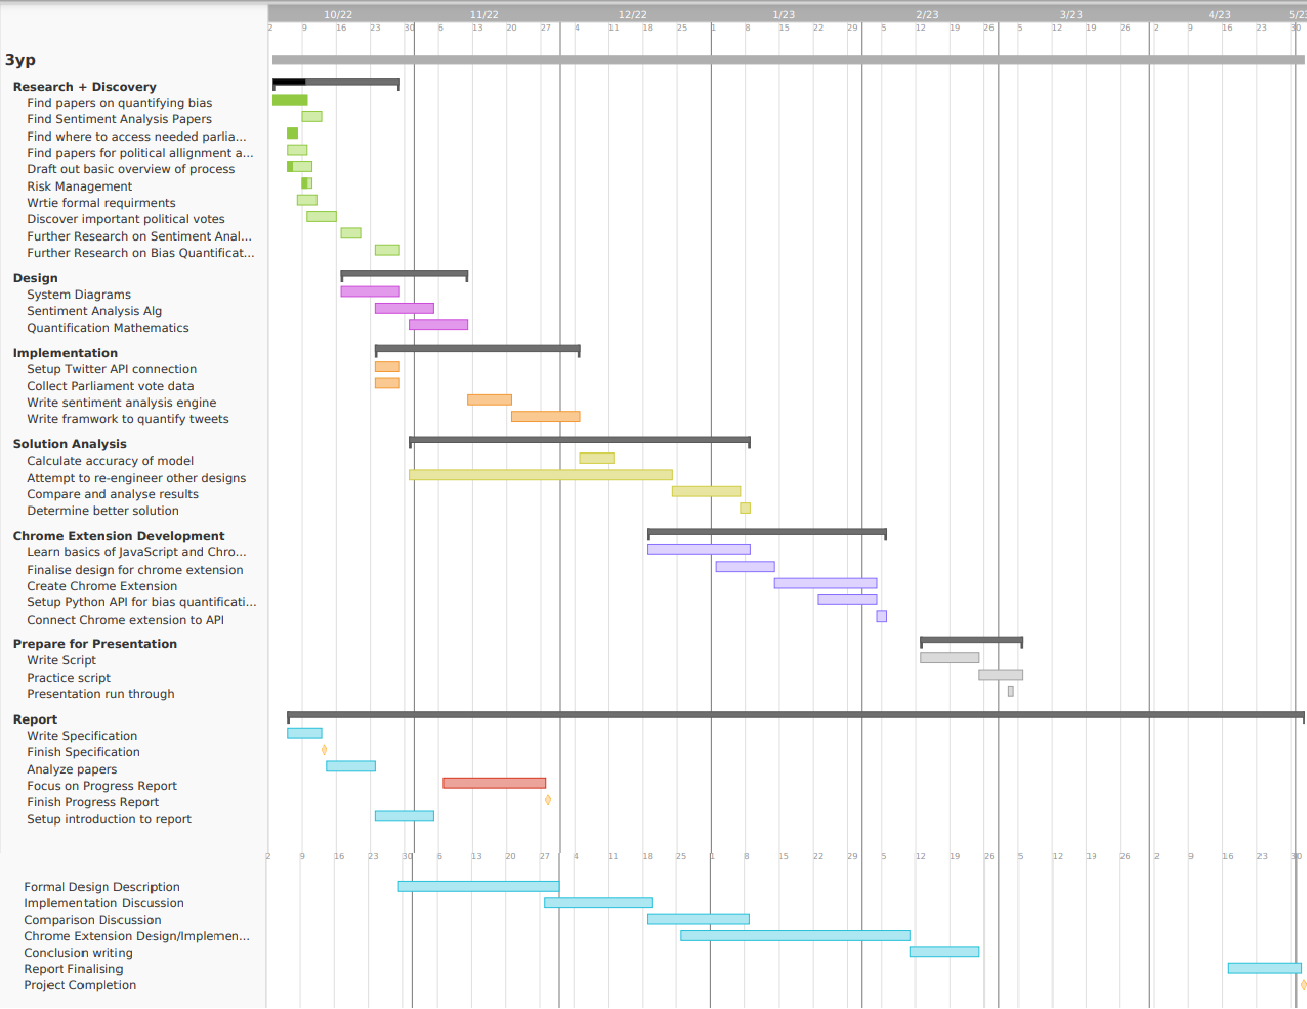
\includegraphics[width=150mm]{../images/3yp timeline.png}
    \caption{Project Timeline}
    \label{fig:timeline}
\end{figure}
\newpage
\section{Risk Management}
There are several factors that pose a risk to this project. Below is a table to illustrate what risks are prevalent, how big of an impact they will have, and how to counteract these risks.\\
The scores are ranked from 1-5. 5=high, 1=low.\\
Also note, the impact is the believed impact

\begin{table}[h]
    \begin{tabular}{|p{25mm}|p{20mm}|p{13mm}|p{55mm}|p{14mm}|}
    \hline
        Risk & Likelihood of Occurring & Impact to Project & Impact Mitigation & New Impact \\
        \hline
        Personal issue causing delay in schedule & 4 & 3 & I have purposefully planned my project with room to & 1 \\
        \hline
        Chosen design philosophy fails to produce useful bias metrics & 3 & 4 & Firstly, this project is mainly research based, so no matter the outcome we will gain something from the comparison between approaches. For the Software side of the project we could instead use an already known method if ours does not work. & 2 \\
        \hline
        Changes to Twitter API & 2 & 1 & Any changes to the API should not dramatically affect this project. At worse it could involve some minor code refactoring to correct endpoints/REST queries. & 1\\
        \hline
        Laptop dies & 1 & 5 & Using git+github for version control throughout this project (for code and report), no matter what happens to my own laptop, the codebase will be accessible from any machine & 1\\
        \hline
    \end{tabular}
    \caption{Possible risks}
    \label{tab:risk}
\end{table}

\bibliographystyle{../common/plainnat}
\bibliography{../common/bibliography}

\end{document}
